% !TeX root = ../../Thesis.tex

\chapter{Inflationary stimulated Raman scattering in shock-ignition plasmas}
\label{chp:iSRS}
\bibliographystyle{plainnat}
\nobibliography*

\title{Inflationary stimulated Raman scattering in shock-ignition plasmas}

This chapter is adapted, with the permission of AIP Publishing, from:
\begin{itemize}
  \item \bibentry{Spencer2020}.
\end{itemize}

\section{Motivation and literature review}
\subsection{Homogeneous plasmas}
\subsection{Inhomogeneous plasmas}


\section{Code and initial conditions}\label{sec:code&IC}
As described in Chapter \ref{chp:methods}, all simulations are performed using the EPOCH \cite{Arber2015} particle-in-cell code. The simulation parameters are chosen to achieve our primary aim of identifying plasma parameters where iSRS may occur, which does not require large simulations of the entire LPI system. The simulations all used a domain size of $L_x = 100\si{\micro\metre} $ and ran to $T_\mathrm{end} = 2\si{\pico\second}$
with 2048
particles per cell (PPC) for the electron species.
We treat the ions as a neutralising background population since we simulate only a two pico-second interval of SRS
development, during which ion dynamics will not become important \cite{Rousseaux2006}.
For the plasma parameters laid out above, electron-ion collisions occur on a characteristic timescale of approximately
$7 \si{\pico\second}$ at the highest density probed, $0.22n_\mathrm{cr}$. Since the inflationary Raman process we
are investigating takes place
on a sub-picosecond timescale, we do not include collisions in our simulations.
The plasma density profiles are given by the expression $n(x) = n_\mathrm{min}\mathrm{exp}(x/L_n)$ and can be seen in Table
\ref{tab:densities}.

We simulate a frequency-tripled Nd:glass laser with vacuum wavelength $\lambda_0 = 351\si{\nano\metre}$, polarised in the $y$-direction. The laser intensity was varied in 20 logarithmically evenly-spaced increme\
nts between $10^{14}$\si{W/\centi\metre^2} and $10^{16}$\si{W/\centi\metre^2}, with a half-Gaussian temporal profile followed by a flat top, and a rise-time of 50 laser periods.
We use absorbing boundaries for the fields and thermal for the particles; these replace any particle leaving the
simulation with an incoming particle with velocity consistent with a Maxwellian plasma based on the initial temperature of $4.5$\si{keV}.

\begin{table}[ht]
    \caption{\label{tab:densities}
        Summary of density profiles and $k_{EPW}\lambda_\mathrm{D}$ values in each simulation. $L_n=n_e/(dn_e/dx)$ evaluated at $n_\mathrm{mid}$. For all but the case centred at $0.2n_\mathrm{cr}$, $k_\mathrm{EPW}\lambda_\mathrm{D} > 0.28$ and we are in the strongly kinetic regime. The total range of $k_\mathrm{EPW}\lambda_\mathrm{D}$ probed is 0.21-0.41.
        }
    %\begin{ruledtabular}
    \begin{center}
    \begin{tabular}{|c|c|c|c|}
    $L_n/\si{\micro \metre}$  & $n_\mathrm{mid}/n_\mathrm{cr}$ & $(n_\mathrm{min},n_\mathrm{max})/n_\mathrm{cr}$ &$(k\lambda_\mathrm{D_{min}},k\lambda_\mathrm{D_{max}})$\\
    \hline
    300& 0.15  & $(0.13,0.18)$ & $(0.28,0.37)$\\
    500 & 0.12 &$(0.11,0.13)$ & $(0.37,0.41)$\\
    500 & 0.15 & $(0.14,0.17)$& $(0.29,0.35)$ \\
    500 & 0.20 & $(0.18,0.22)$& $(0.21,0.27)$\\
    1000 & 0.15 & $(0.14,0.16)$ & $(0.31,0.32)$ \\
    \end{tabular}
    \end{center}
    %\end{ruledtabular}
\end{table}

\section{Diagnosing iSRS in inhomogeneous plasmas}\label{sec:signatures}
\subsection{Inflation threshold}

\begin{figure}[ht]
    \centering
    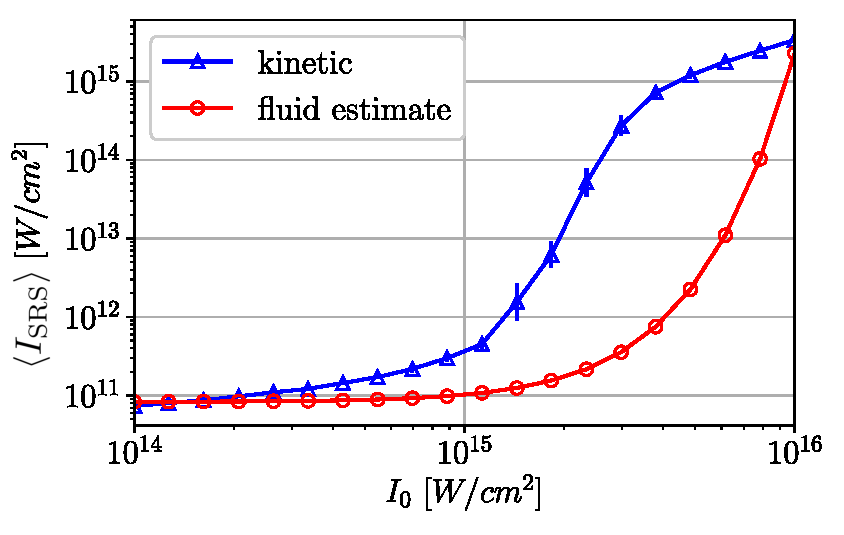
\includegraphics[width=0.8\columnwidth]{Chapters/C4_iSRS/fig2.pdf}
    \caption{
        Blue triangular markers show the intensity of SRS scattered light calculated using the fully-kinetic EPOCH code for parameters: $L_n = 500 \si{\micro\metre} $ and $n_{\mathrm{mid}} = 0.15n_\mathrm{cr}$.
        Red circular markers show the intensity of SRS scattered light calculated, for the same plasma parameters, from the fluid model presented above.
        The initial noise level in the fluid model was calculated from a PIC simulation without the laser driver: $I_\mathrm{noise}=\langle E_yB_z\rangle_{x,t} / \mu_0 = 8\times 10^{10} \si{W/\centi\metre^2}$.}
    \label{fig:kineticVsfluid}
\end{figure}{}

\subsection{Electron trapping}
\begin{figure}[!ht]
 \centering
 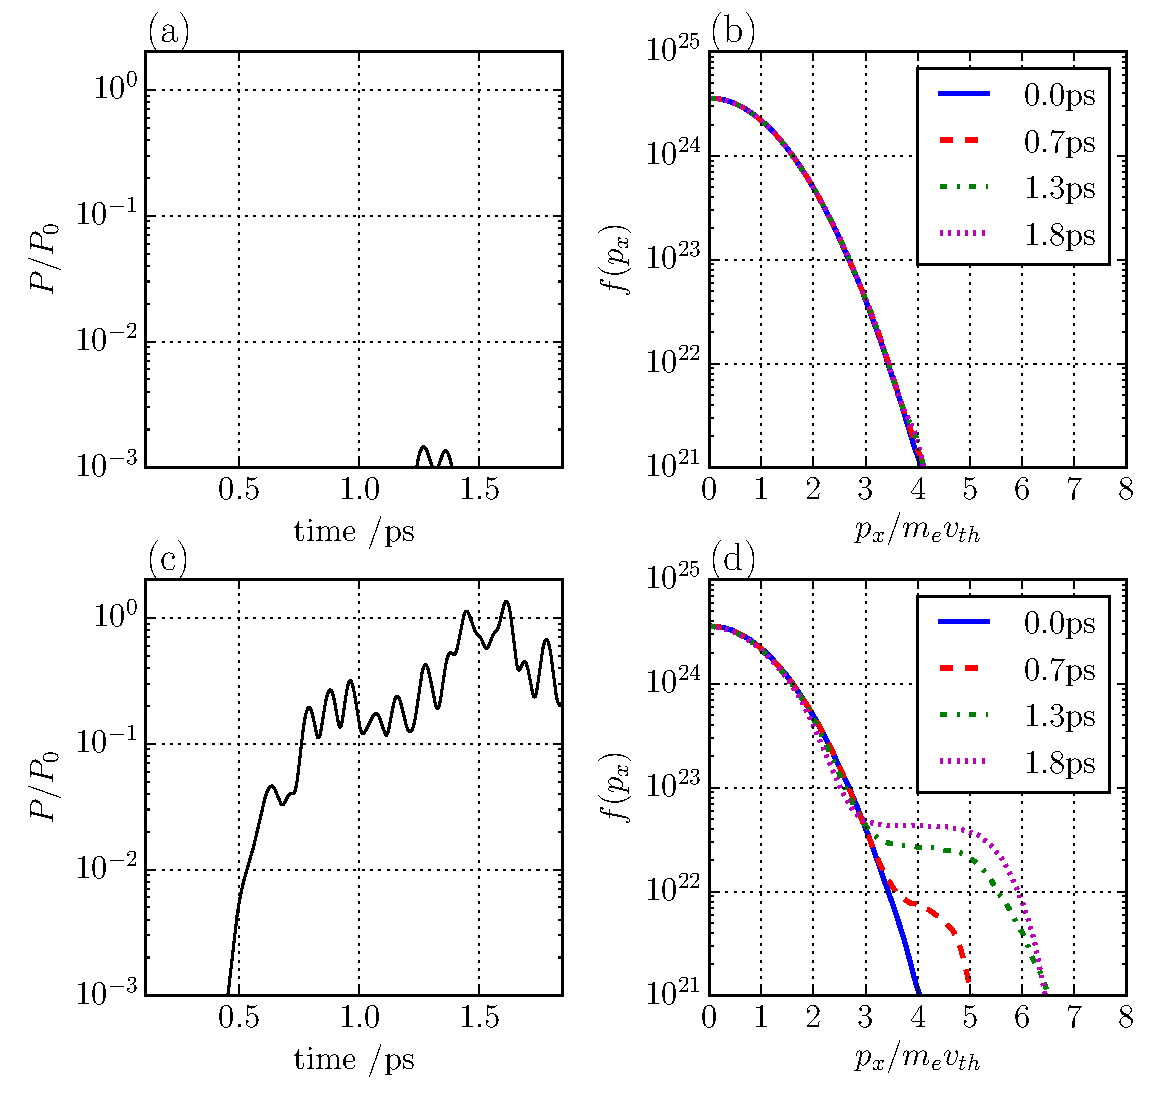
\includegraphics[width=0.7\columnwidth]{Chapters/C4_iSRS/fig3_3a_3b_3c_3d.pdf}
 \caption{Time-resolved comparison of SRS-reflectivity (a,c) and electron distribution 
 functions (b,d) for two simulations with parameters: $L_n = 500 \si{\micro\metre} $; centred
 at $0.15n_\mathrm{cr}$; and $T_e = 4.5$\si{\kilo\electronvolt}. The distribution function of
 electron momentum is averaged over the entire spatial domain at four times, normalised to the initial thermal momentum. Panels (a,b) have an incident laser intensity below the threshold for inflationary SRS; $I_0 = 1.13\times10^{15}$\si{W/\centi\metre^2}. Panels (c,d) have an incident laser intensity above the iSRS threshold; $I_0 = 4.83\times10^{15}$\si{W/\centi\metre^2}.}
 \label{fig:reflAndDist}
\end{figure}

A second signature of iSRS, as reported in the literature for homogeneous plasmas, is electron-trapping in the SRS electron plasma waves, leading to a
non-linear frequency shift and enhanced SRS-reflectivies at large $k\lambda_\mathrm{D}$ \cite{Vu2002}.
A typical manifestation of this, for our inhomogeneous simulations, is shown in Figure \ref{fig:reflAndDist}. Figure \ref{fig:reflAndDist}
shows the instantaneous SRS-reflectivity measured at the left boundary of the simulation domain (a,c), alongside the box-averaged electron
distribution function at four times (b,d), for two simulations with laser intensities above and below the iSRS threshold.
Sub-figures \ref{fig:reflAndDist} (a,b) show that, when driven below threshold, the distribution of electron momenta is Maxwellian throughout the simulation, and that the maximum instantaneous power in SRS-refle\
cted light is consequently very low ($P \sim 10^{-3}P_0$). In sub-figures (c,d), where the incident laser intensity is well above the iSRS threshold, we see that the power in SRS-reflected light is correlated wi\
th the growth of a non-Maxwellian tail in the distribution function, corresponding to an electron population trapped in the SRS electron plasma waves.
There is a general trend of increasing SRS-reflected light that correlates with
the increasing trapped electron population.


\subsection{Nonlinear frequency shift}
\begin{figure}[h!]
    \centering
    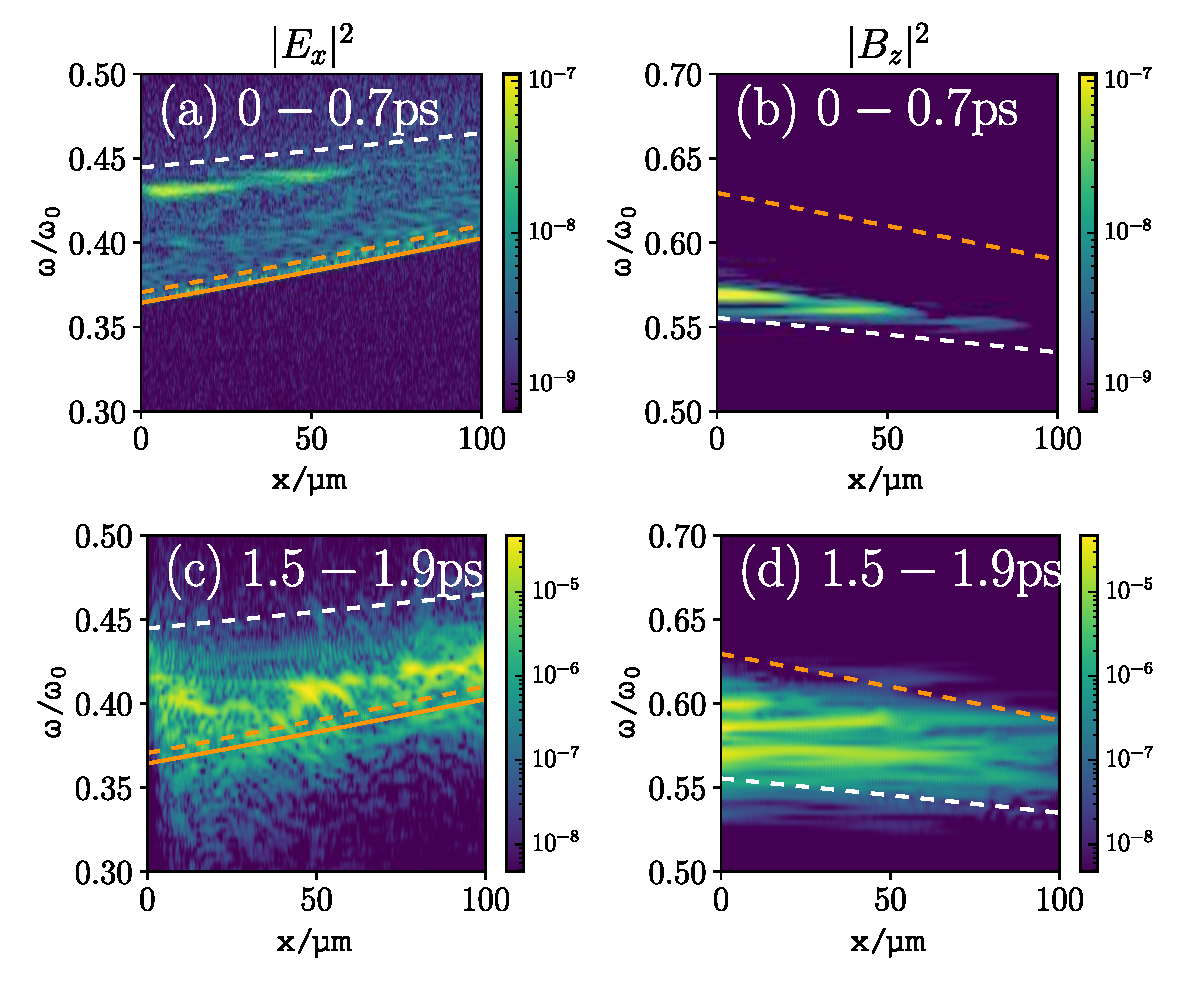
\includegraphics[width=0.9\columnwidth]{Chapters/C4_iSRS/fig4_4a_4b_4c_4d.pdf}
    \caption{Top panels show the spectra of electrostatic (a) and electromagnetic (b) waves over the period $0-0.7\si{\pico\second}$.
    The white (orange) dashed lines represent the linear predictions for the spectra of backward (forward) SRS. The bottom panels show the same spectra calculated over the period $1.5-1.9\si{\pico\second}$. The \
$E_x$ ($B_z$)
    spectrum is significantly down-shifted (up-shifted), demonstrating a trapped population of electrons in the EPW \cite{Yin2006}.
    The orange solid line represents the plasma frequency $\omega_{\mathrm{pe}}$ for the simulation parameters: $L_n = 500 \si{\micro\metre} $ centred at $0.15n_\mathrm{cr}$ and $I_0 = 4.83\times10^{15}$\si{W/\c\
enti\metre^2}.}
    \label{fig:downshift}
\end{figure}{}


\subsection{Beam acoustic modes}
\begin{figure}[ht]
    \centering
    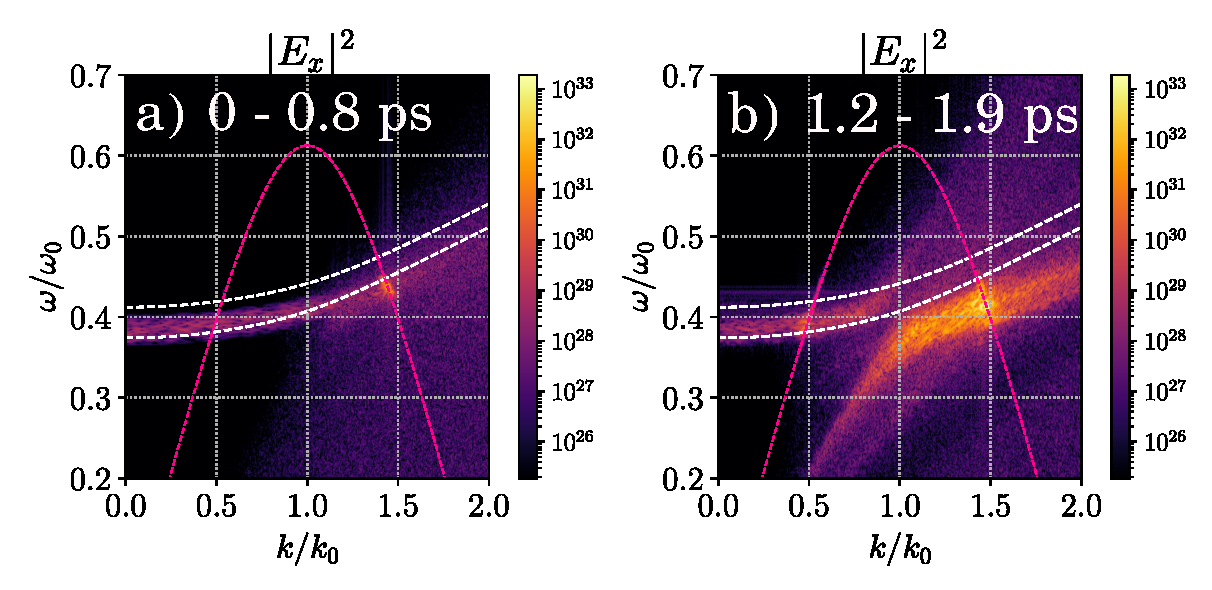
\includegraphics[width=0.8\columnwidth]{Chapters/C4_iSRS/fig5_5a_5b.pdf}
    \caption{(Colour) (a) 2D FFT of $E_x$ over the period $ 0 - 0.8 \si{\pico\second}$. (b) 2D FFT of $E_x$ over the period $1.2 - 1.9                                                                              
    \si{\pico\second}$.
    The white dashed lines represent the analytical dispersion relations corresponding to the minimum (bottom line) and maximum (top line) plasma densities,
    assuming a Maxwellian electron distribution.
    The pink dashed line shows the Stokes line for down-shifted EM waves.
    Simulation parameters: $L_n = 500 \si{\micro\metre} $ centred at $0.15n_\mathrm{cr}$
    and $I_0 = 4.83\times10^{15} \si{W/\centi\metre^2}$.
    }
    \label{fig:BAM}
\end{figure}{}


%%%%%%%%%%%%%%%%%%%%%%%%%%%%%%%%%%%%%%%%%%%%%%%%%%%%%%%%%%%%%%%%%%%%%%%%%%%%%%%%%%%%%%%%%%
%%                              SEC: THRESHOLD AND HE                                   %%
%%%%%%%%%%%%%%%%%%%%%%%%%%%%%%%%%%%%%%%%%%%%%%%%%%%%%%%%%%%%%%%%%%%%%%%%%%%%%%%%%%%%%%%%%%

\section{Intensity threshold and hot electron scaling}\label{sec:paramScan}

\begin{figure}[!ht]
     \centering
    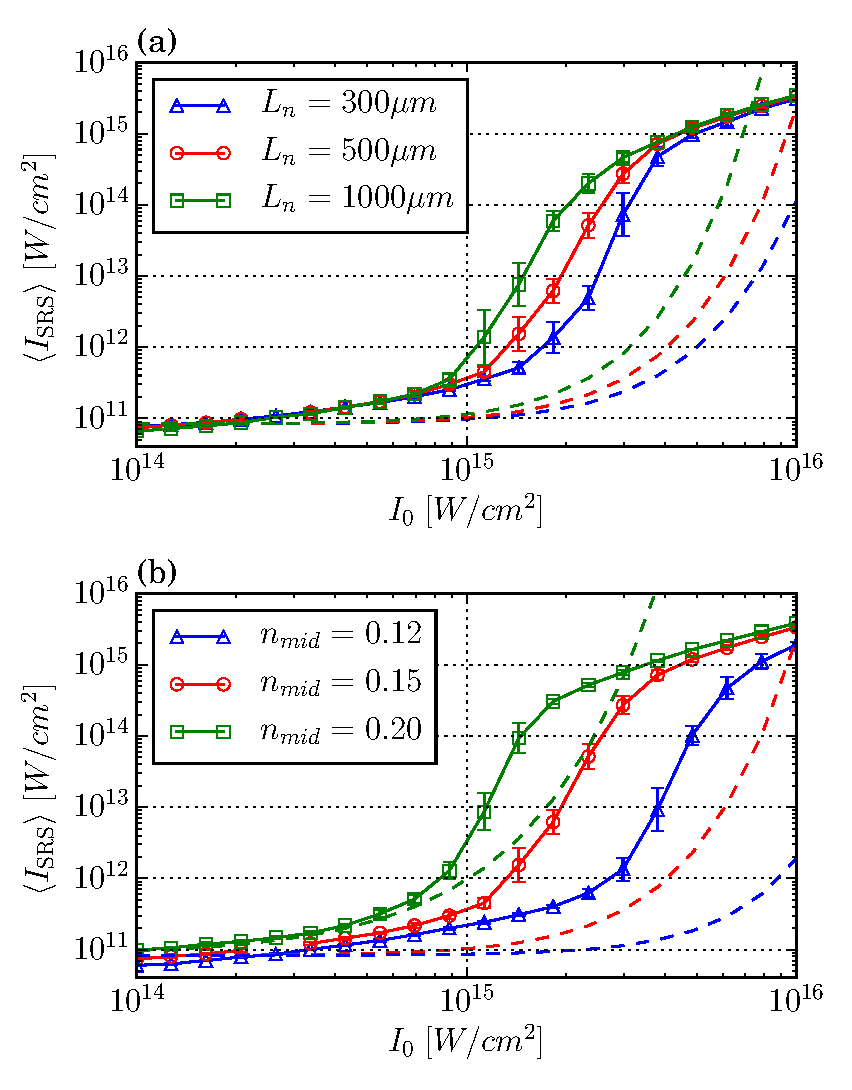
\includegraphics[width=0.5\columnwidth]{Chapters/C4_iSRS/fig6_6a_6b.pdf}
    \caption{
    (Colour) (a)  Relationship between incident laser intensity and the intensity of SRS scattered light for three different density scale-lengths, with plasma density profiles centred at $0.15n_\mathrm{cr}$.
    (b) Relationship between incident laser intensity and the intensity of SRS scattered light for three simulations with $L_n=500\si{\micro\metre}$ centred at three different densities.
    Each coloured dashed line represents the prediction of the fluid model presented in Section \ref{sec:signatures} for the same parameters as the solid line of the same colour.
    }
    \label{fig:paramScan}
\end{figure}


\section{Saturation}
In all of the 

\section{Conclusion}\label{sec:conclusion}

\bibliography{Chapters/C4_iSRS/iSRS}
